\documentclass[9pt]{beamer}

\usepackage{appendixnumberbeamer}
\usepackage{booktabs}
\usepackage[scale=2]{ccicons}
\usepackage{pgfplots}
\usepackage{tikz}
\usepackage{graphics}
\usepackage{chemfig}

\usepgfplotslibrary{dateplot}
\pdfstringdefDisableCommands{\def\translate#1{#1}}
\geometry{paperwidth=140mm, paperheight=105mm}
\usetheme{metropolis}
\bibliographystyle{abbrv}
\setbeamertemplate{frame footer}{ME663 - Computational Fluid Dynamics}

\usetikzlibrary{shapes, arrows}
\tikzstyle{startstop} = [rectangle, rounded corners, minimum width=2cm, minimum height=1cm, text centered, draw=black, fill=red!30]
\tikzstyle{io} = [trapezium, trapezium stretches=true, trapezium left angle=70, trapezium right angle=110, minimum width=2cm, minimum height=1cm, text centered, draw=black, fill=blue!30]
\tikzstyle{process} = [rectangle, minimum width=2cm, minimum height=1cm, text centered, text width=2cm, draw=black, fill=orange!30]
\tikzstyle{decision} = [diamond, minimum width=2cm, minimum height=1cm, text centered, draw=black, fill=green!30]
\tikzstyle{arrow} = [thick,->,>=stealth]

\title{Designing a Suitable Fuel Injector for Ammonia Using CFD}
\subtitle{Next-Generation Fuel in Internal Combustion Engine}
\date{March 20, 2024}
\author{Tommaso Bocchietti}
\institute{University of Waterloo}
\titlegraphic{\hfill
\includegraphics[height=1.5cm]{pdf/UniversityOfWaterloo_logo_horiz_pms.pdf}}

\begin{document}

\maketitle\begin{frame}{Agenda}
    \setbeamertemplate{section in toc}[sections numbered]
    \tableofcontents[hideallsubsections]
\end{frame}

\section{Motivations}

\begin{frame}{$\mathrm{CO_2}$ Emission by Sector}

    Transportation sector is the second-largest contributor to $\mathrm{CO_2}$ emission.

    \vspace{9pt}

    \begin{figure}
        \centering
        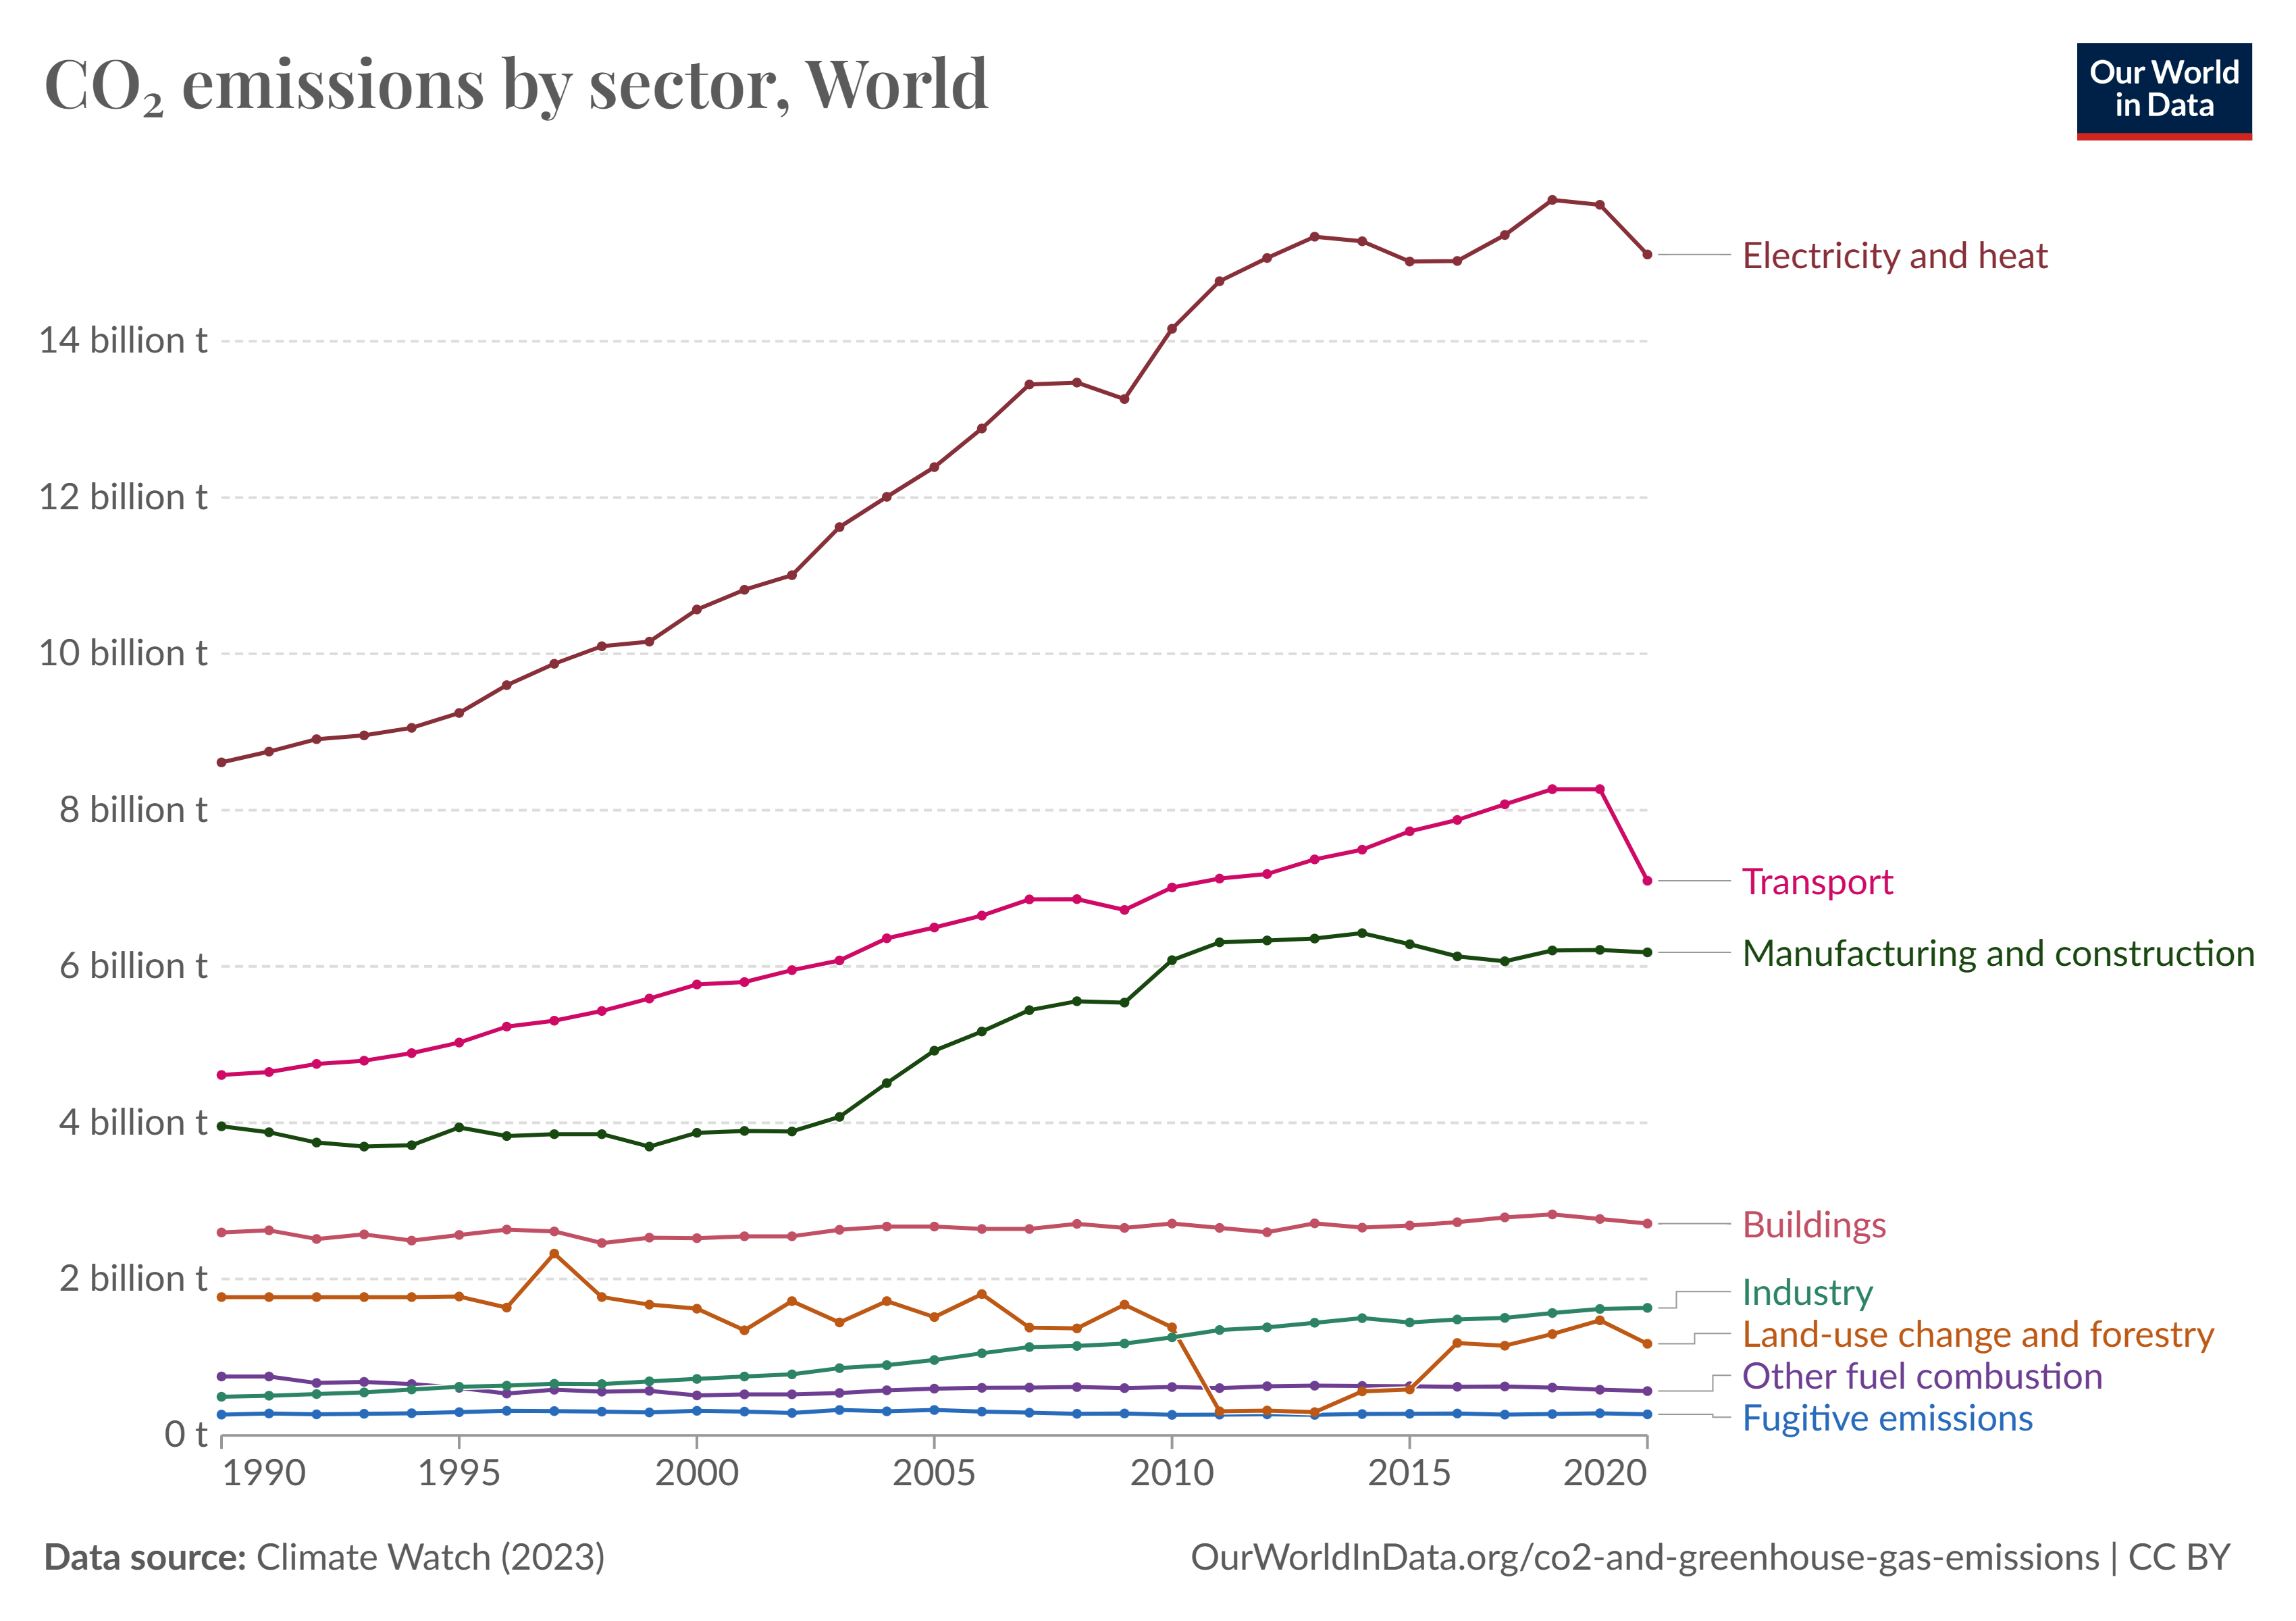
\includegraphics[width=0.8\textwidth]{img/co-emissions-by-sector.png}
        % \caption{$\mathrm{CO_2}$ Emission by sector}
    \end{figure}

\end{frame}



\begin{frame}{Alternative to traditional Fossil Fuel}

    Transportation sector has been looking for alternative fuels to reduce $\mathrm{CO_2}$ emission.

    \begin{itemize}
        \item \textbf{Electricity:} requires a large infrastructure to support the global demand
        \item \textbf{Methane:} worse than $\mathrm{CO_2}$ in terms of greenhouse effect (short-term)
        \item \textbf{Hydrogen:} difficult to store and transport
    \end{itemize}

\end{frame}



\begin{frame}{Ammonia as a Fuel}

    Researchers started looking at Ammonia as a potential alternative fuel.

    \vspace{9pt}

    \begin{columns}[c, onlytextwidth]

        \begin{column}{0.45\textwidth}

            \begin{figure}[H]
                \centering

                \LARGE
                \setchemfig{atom sep=5em, bond offset=5pt}
                \chemfig{\charge{90=\:}{N}(-[:210]H)(<[:290]H)(<:[:-15]H)}
                \normalsize

                \caption{Ammonia molecule ($\mathrm{NH_3}$)}

            \end{figure}

        \end{column}

        \begin{column}{0.55\textwidth}

            Advantages of Ammonia:

            \begin{itemize}
                \item No carbon content (zero $\mathrm{CO_2}$ emission)
                \item Long history of use in the chemical industry
                \item Possible use as hydrogen carrier
            \end{itemize}

        \end{column}

    \end{columns}

\end{frame}



\begin{frame}{Ammonia as a Fuel}

    \begin{columns}[c, onlytextwidth]

        \begin{column}{0.33\textwidth}

            \begin{figure}[H]
                \centering
                
\includegraphics[width=0.5\textwidth]{pdf/nfpa-diesel.pdf}
            \end{figure}

        \end{column}

        \begin{column}{0.33\textwidth}

            \begin{figure}[H]
                \centering
                
\includegraphics[width=0.5\textwidth]{pdf/nfpa-gasoline.pdf}
            \end{figure}

        \end{column}

        \begin{column}{0.33\textwidth}

            \begin{figure}[H]
                \centering
                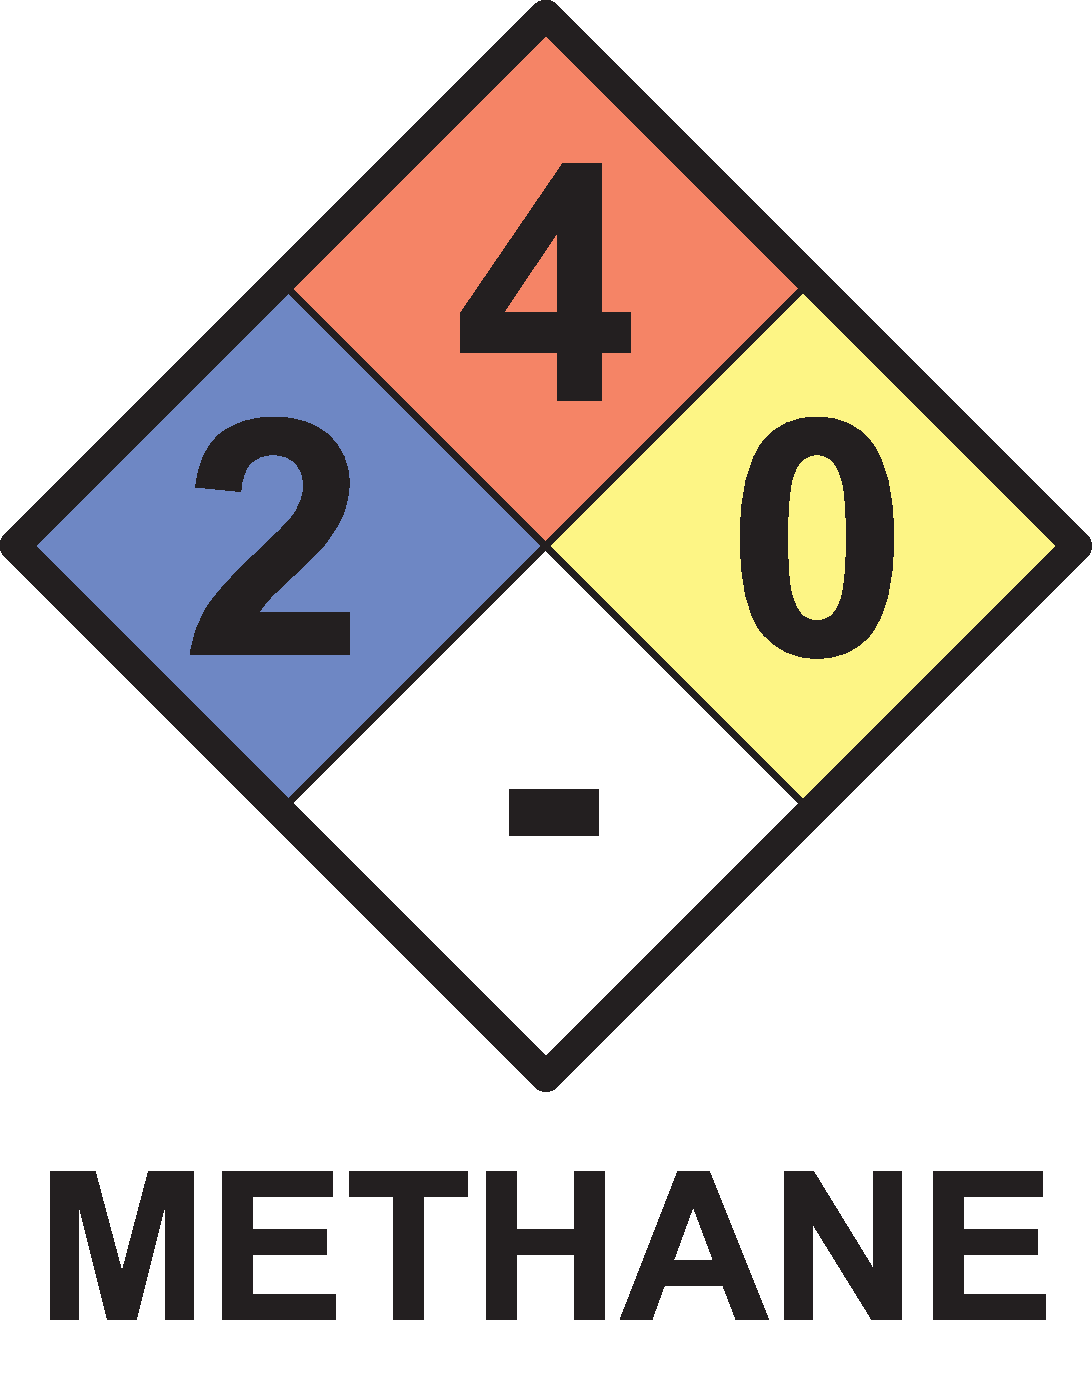
\includegraphics[width=0.5\textwidth]{pdf/nfpa-methane.pdf}
            \end{figure}

        \end{column}

    \end{columns}

    \begin{columns}[c, onlytextwidth]

        \begin{column}{0.4\textwidth}

            \begin{figure}[H]
                \centering
                
\includegraphics[width=0.5\textwidth]{pdf/nfpa-ammonia.pdf}
            \end{figure}

        \end{column}

        \begin{column}{0.6\textwidth}

            Disadvantages of Ammonia (also based on NFPAs\footnotemark[1]):

            \begin{itemize}
                \item Least flammable source, which also suggest \textbf{slow flame speed}
                \item Its combustion might produce \textbf{high $\mathrm{NO_x}$ emissions} if not properly controlled
                      % \item High ignition temperature
                      % Low flame velocity
                      % Slow chemical kinetics
            \end{itemize}

        \end{column}

    \end{columns}

    \footnotetext[1]{National Fire Protection Association 704: Standard System for the Identification of the Hazards of Materials for Emergency Response}

\end{frame}
\section{Research Focus}

\begin{frame}{Fuel injector for Ammonia}

    \begin{columns}[c, onlytextwidth]

        \begin{column}{0.5\textwidth}

            Design a \textbf{direct Ammonia fuel injector compatible with current internal combustion engines}.

            \vspace{9pt}

            The key factors driving our design will be:

            \begin{itemize}
                \item Stable flame inside the combustion chamber
                \item Low-to-zero $\mathrm{NO_x}$ emissions
            \end{itemize}

        \end{column}

        \begin{column}{0.5\textwidth}

            \begin{figure}[H]
                \centering
                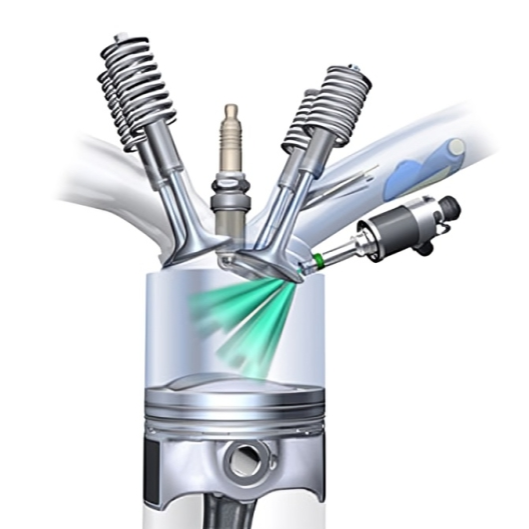
\includegraphics[width=0.9\textwidth]{img/injectors-in-ICE.png}
                \caption{Direct fuel injection in internal combustion engines}
            \end{figure}

        \end{column}

    \end{columns}

\end{frame}



\begin{frame}{Fuel injector for Ammonia}

    \begin{columns}[c, onlytextwidth]

        \begin{column}{0.4\textwidth}

            \begin{figure}[H]
                \centering
                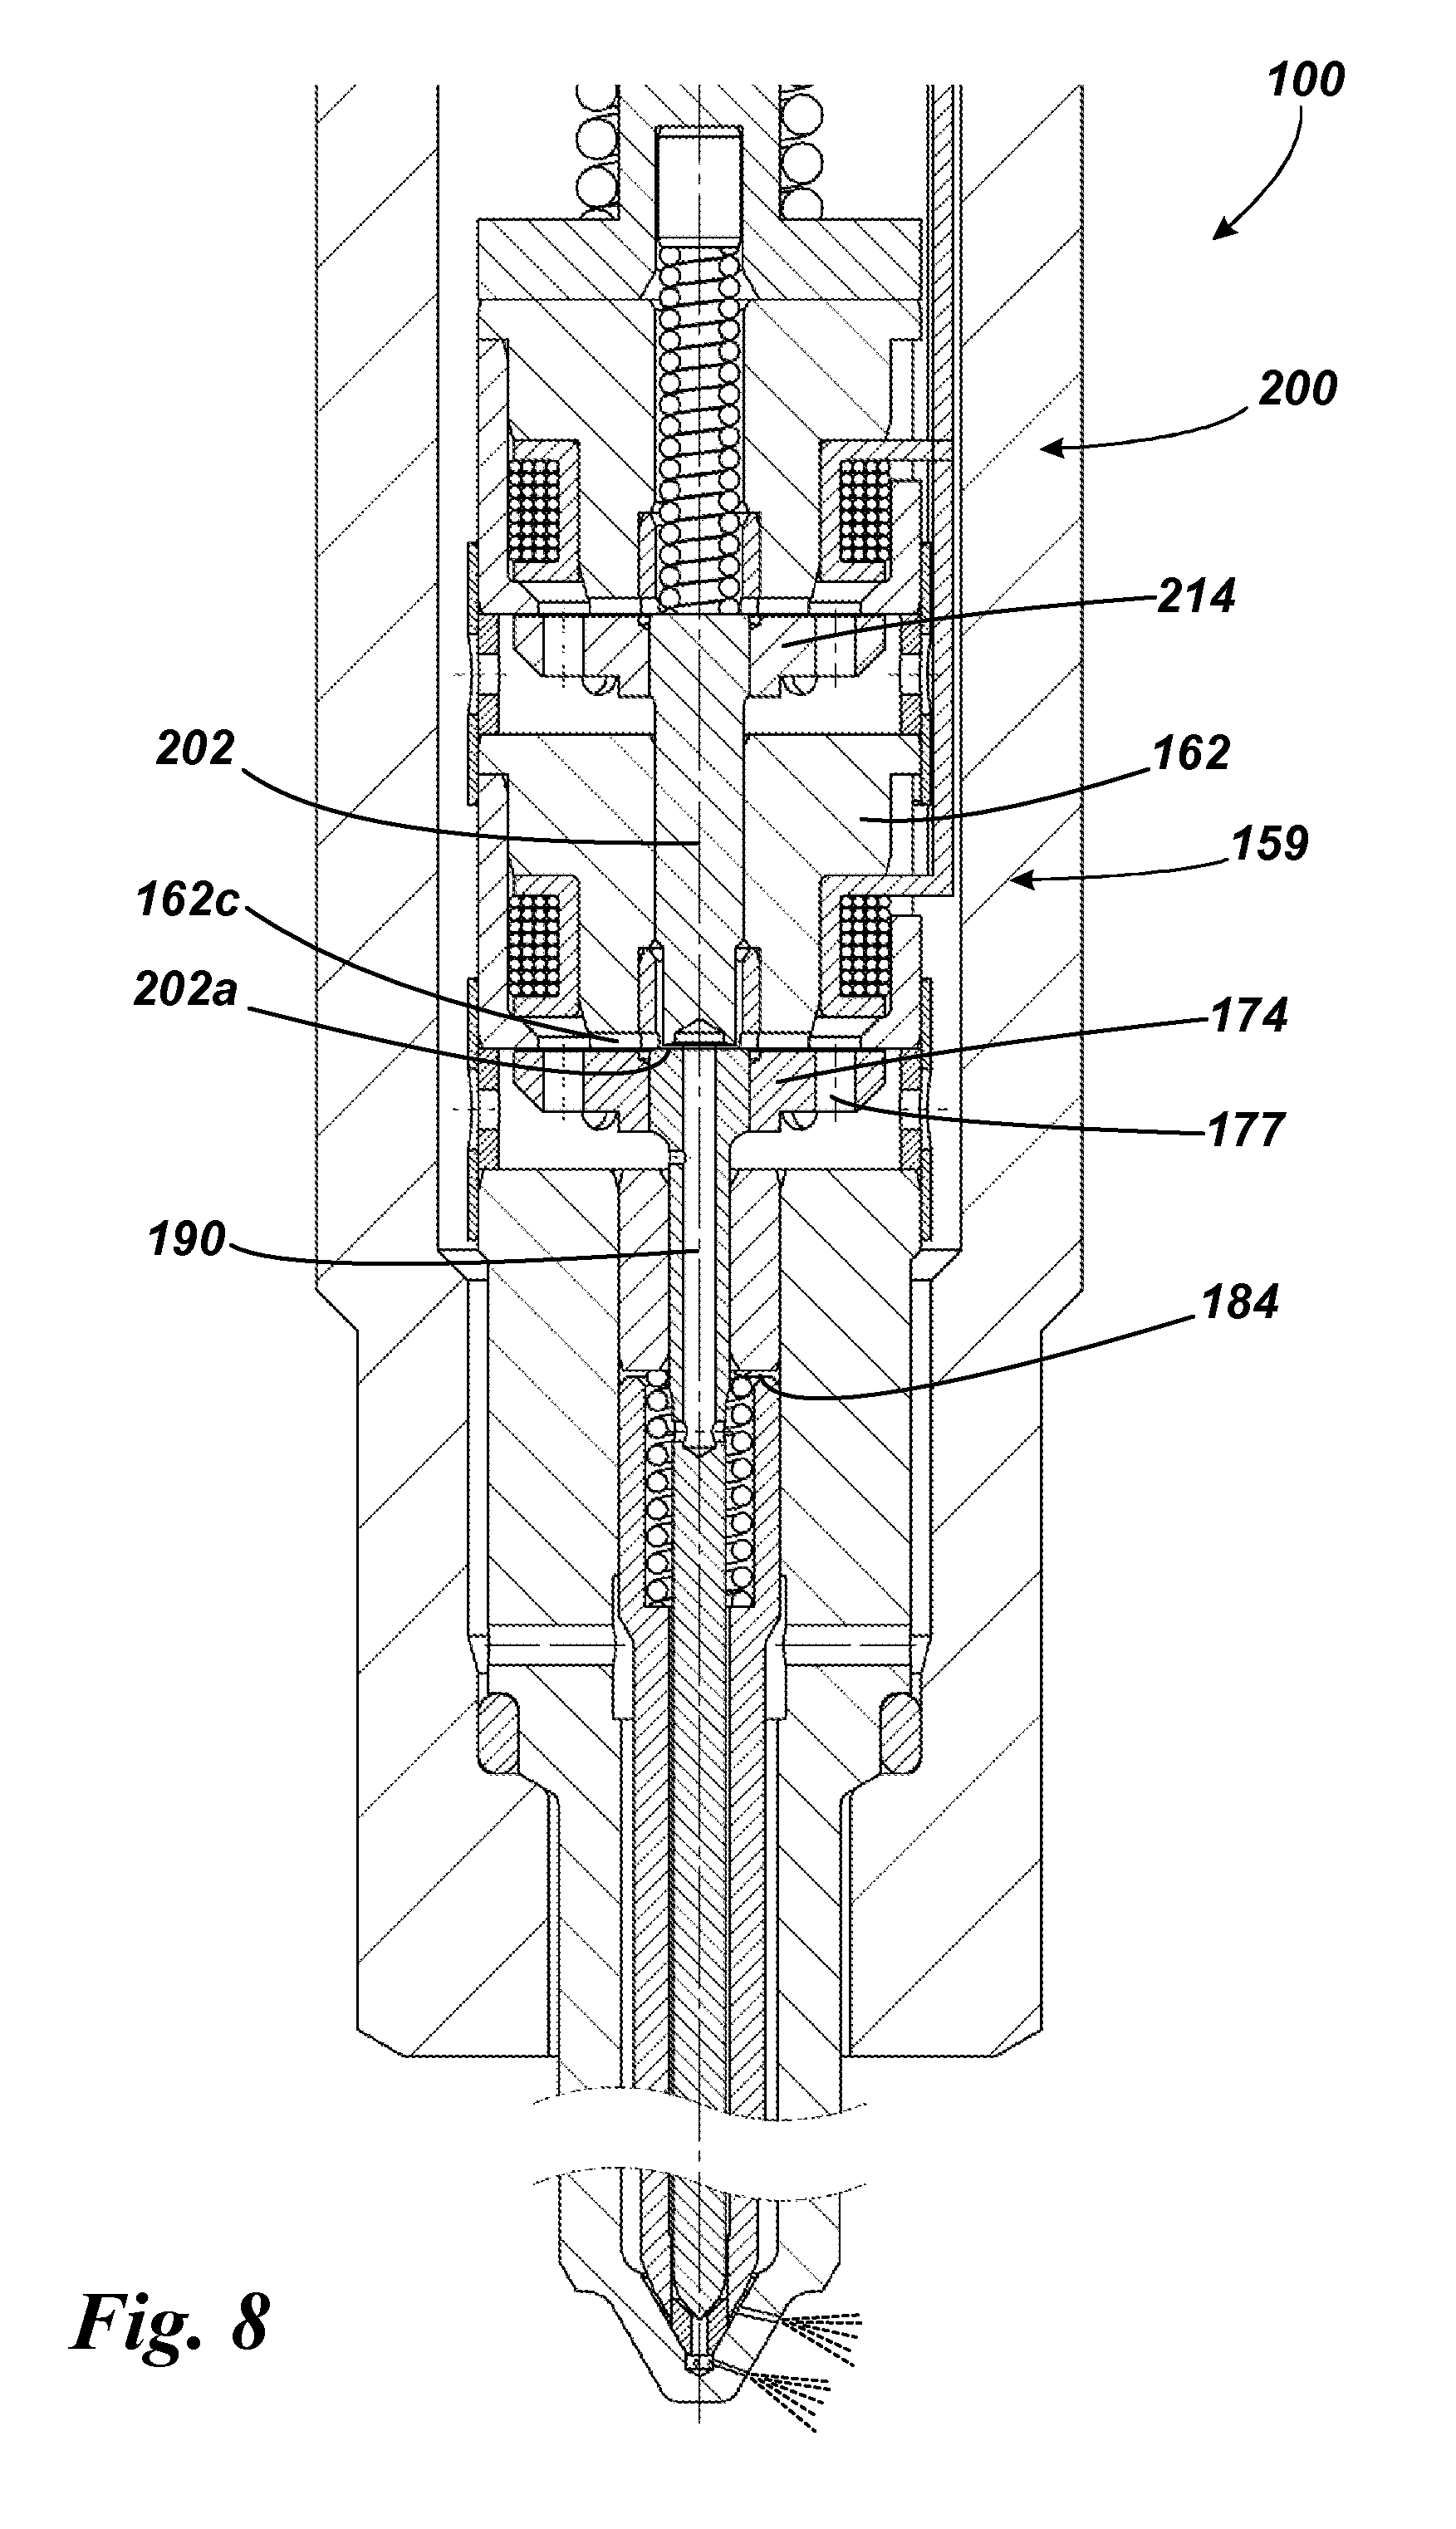
\includegraphics[width=0.8\textwidth]{img/injector-drawing.png}
                \caption{"Fuel injector" (US20120080011A1)}
            \end{figure}

        \end{column}

        \begin{column}{0.6\textwidth}

            The core focus will be on the \textbf{controllability of the atomization process}.

            \vspace{9pt}

            Given that, we also need to take into account the environmental working conditions:

            \begin{itemize}
                \item Temperatures (inlet, chamber, exhaust)
                \item Pressures (inlet, chamber, exhaust)
                \item Air-fuel ratio
                \item Injection timing
            \end{itemize}

        \end{column}

    \end{columns}

\end{frame}
\section{Prior Studies}

\begin{frame}{2021 - R. Pelé et al.}

    Title: First Study on Ammonia Spray Characteristics with a Current GDI Engine Injector

    \vspace{9pt}

    \begin{columns}[c, onlytextwidth]

        \begin{column}{0.45\textwidth}

            \begin{figure}[H]
                \centering
                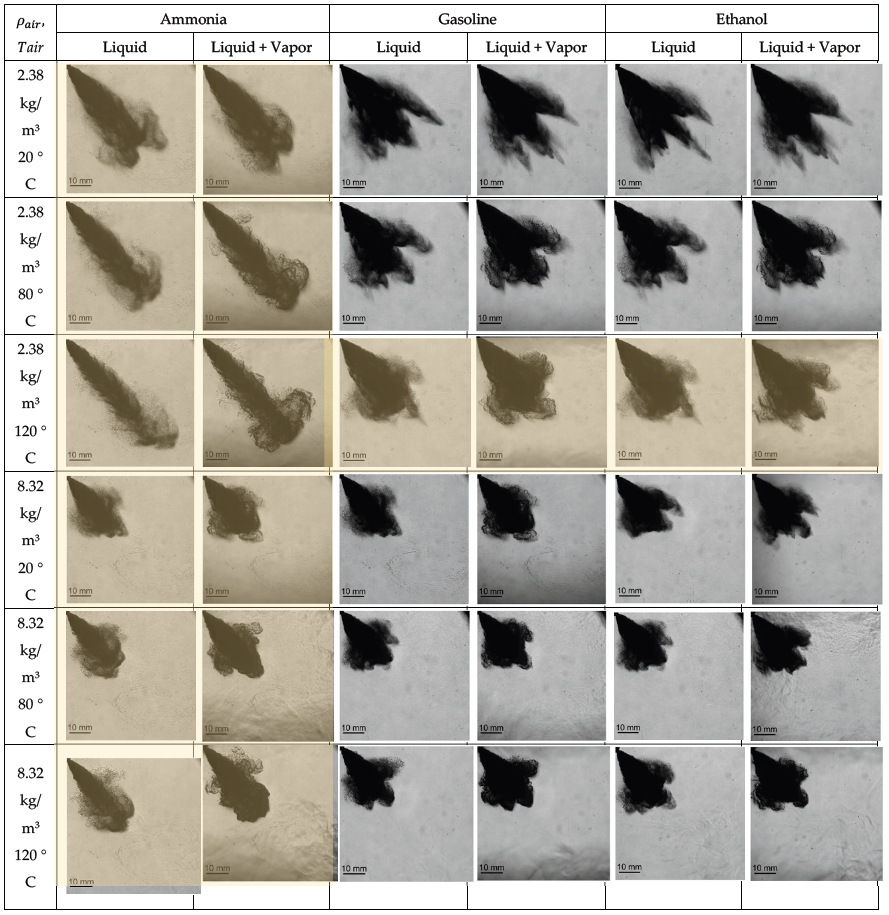
\includegraphics[width=0.8\textwidth]{img/studies-Pele.png}
                \caption{Comparison of spray shape (different fuels \& conditions).}
            \end{figure}

        \end{column}

        \begin{column}{0.5\textwidth}

            Geometrical spray characteristics analysis of Ammonia compared to Gasoline \& Ethanol.

            Conclusions:
            \begin{itemize}
                \item Ammonia spray is longer and thinner.
                \item Spray angle maximum at $P_{sat}$.
                \item Empirical correlation for $spray_L(t)$ proposed.
            \end{itemize}

            In general, the study \textbf{enhanced the possibility for the use of Ammonia} in GDI engines.

        \end{column}

    \end{columns}

\end{frame}



% \begin{frame}{2021 - Y. Fan et al.}
%     Title: Characteristics of Ammonia Spray Injected by Pressure-Swirl Atomizers
% \end{frame}



\begin{frame}{2021 - K.D.K.A. Somarathne et al.}

    Title: Liquid Ammonia Spray Combustion and Emission Characteristics with Gaseous Hydrogen/air Co-firing

    A \textbf{numerical model} for $\mathrm{LNH_3}$\footnotemark[1] combustion was developed and validated (LES\footnotemark[2] based).
    Particular attention to the \textbf{flash-boiling condition} modelling was given.

    \vspace{9pt}

    \begin{figure}[H]
        \centering
        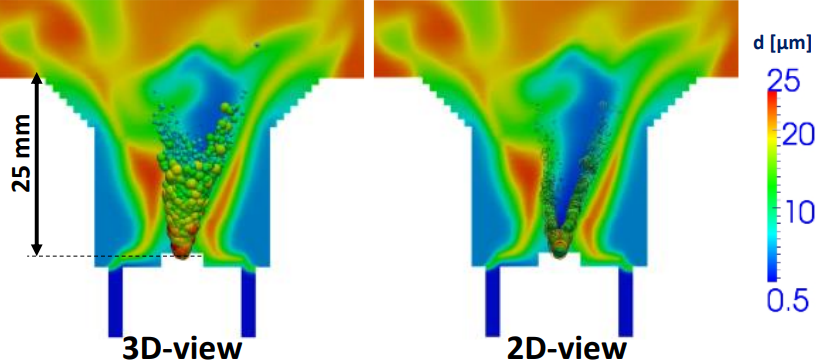
\includegraphics[width=0.6\textwidth]{img/studies-Somarathne.png}
        \caption{3D and 2D views of $\mathrm{LNH_3}$ droplet distributions.}
    \end{figure}

    \footnotetext[1]{LNH3: Liquid Ammonia}
    \footnotetext[2]{LES: Large Eddy Simulation}

\end{frame}



\begin{frame}{2023 - J. Wang, F. Dalla Barba}

    Title: Assessment of the parcel model in evaporating turbulent diluted sprays within a Large-Eddy-Simulation approach

    The \textbf{parcel model} approach was proven to be accurate up to a threshold of the PR\footnotemark[1] number dependent also from the coarsening factor of the grid.

    \vspace{9pt}

    \begin{figure}[H]
        \centering
        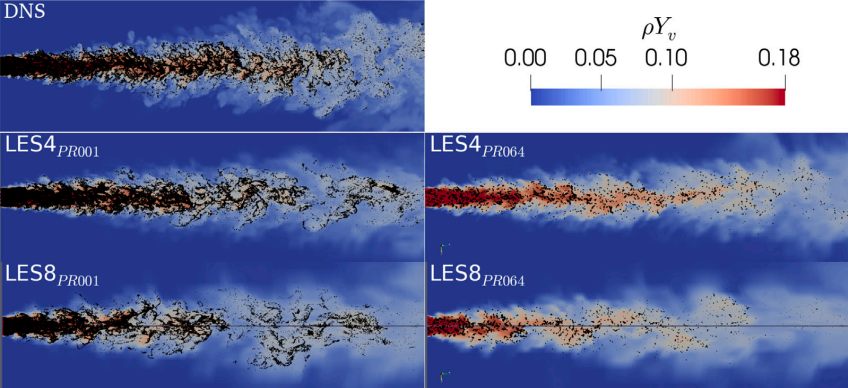
\includegraphics[width=0.8\textwidth]{img/studies-Wang-Dalla-Barba.png}
        \caption{Subset of the simulation runs\footnotemark[2].}
    \end{figure}

    \footnotetext[1]{PR: Parcel Ratio}
    \footnotetext[2]{Here the carrier phase is contoured according to the instantaneous vapor mass fraction field ($\rho Y_v$)}

\end{frame}



\begin{frame}{2023 - J. Wang, F. Dalla Barba}

    The research focused on \textbf{simulating a turbulent diluted acetone jet-spray}.

    \begin{columns}[c, onlytextwidth]

        \begin{column}{0.5\textwidth}

            The numerical model was based on:

            \begin{itemize}
                \item LES framework to simulate turbulence behavior
                \item Hybrid \textbf{Eulerian-Lagrangian technique with two-way coupling}
                \item Parcel model for relaxed droplet tracking
            \end{itemize}

        \end{column}

        \begin{column}{0.5\textwidth}

            \begin{figure}[H]
                \centering
                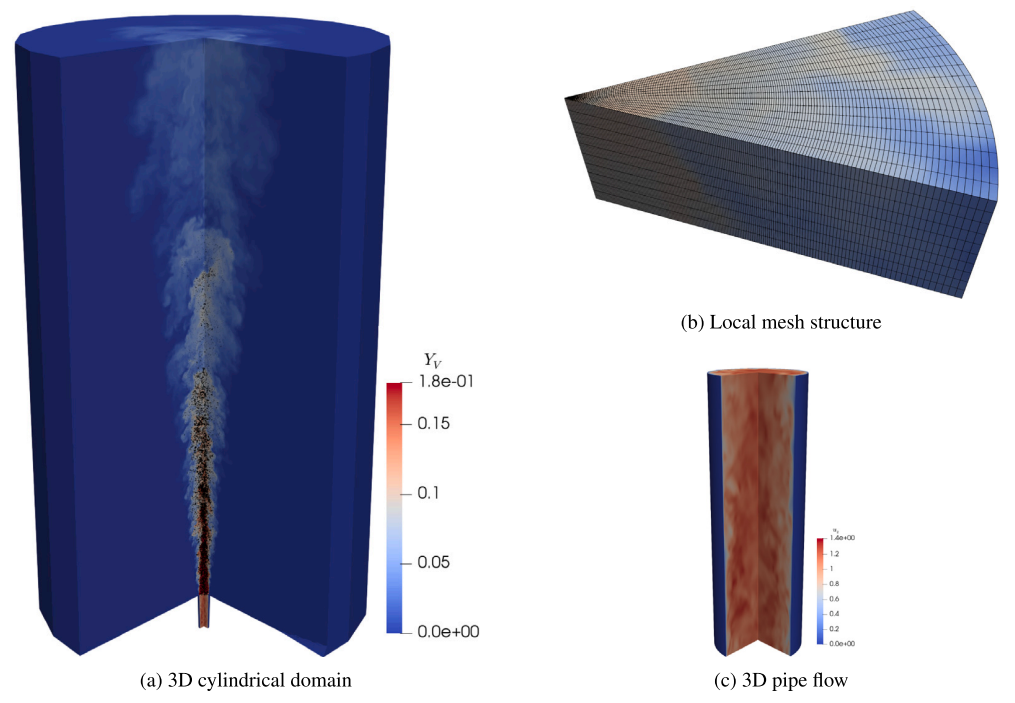
\includegraphics[width=0.9\textwidth]{img/studies-Wang-Dalla-Barba-domain.png}
                \caption{The open-constant pressure-cylindrical domain used for the analysis.}
            \end{figure}

        \end{column}

    \end{columns}

\end{frame}
\section{Methodology}

\begin{frame}{Phase 1.1 - Literature Review}

    A deep literature review to \textbf{better understand the state of the art in Ammonia combustion and the challenges associated with it} will be conducted.
    We will focus on the following topics:

    \begin{itemize}
        \item Combustion dynamics in ICE\footnotemark[1] (flow engineering).
        \item Combustion modeling and CFD\footnotemark[2] simulation for traditional fuels.
        \item Advanced and \textbf{optimized algorithms for numerical simulation of a two-phase dispersed turbulent flow}.
        \item Pollution and emissions from Ammonia derivate combustion products.
    \end{itemize}

    For our research, we will use \texttt{ScienceDirect}, \texttt{Scopus}, \texttt{IEEE Xplore} as main databases.

    A non-exhaustive list of applicable keywords: \textit{Ammonia, Combustion, two-phase dispersed turbulent flow, flash-boiling condition, ICE, CFD}.

    \footnotetext[1]{ICE: Internal Combustion Engine}
    \footnotetext[2]{CFD: Computational Fluid Dynamics}

\end{frame}



\begin{frame}{Phase 1.2 - Model Development}

    An \textbf{accurate and reliable model for Ammonia dynamics (non-reactive)} will be developed starting from previous knowledge of the literature review and experimental data founds.

    From a first analysis of the physics of the problem, we can expect our CFD model to be based on:

    \begin{itemize}
        \item An \textbf{Eulerian algorithm} dedicated to \textbf{advance in time the flow fields} by solving the Low-Mach number formulations of the Navier-Stokes equations
        \item A \textbf{Lagrangian solver} designed to synchronously \textbf{evolve the mass, momentum, and temperature equations} of dispersed droplets under point-particle approximation.
    \end{itemize}

    The model will be developed in \texttt{OpenFOAM} and \texttt{Chemkin}.

\end{frame}



\begin{frame}{Phase 1.3 - Model Validation}

    The model will be \textbf{validated using experimental data} from the literature.

    \vspace{9pt}

    \begin{columns}[c, onlytextwidth]

        \begin{column}{0.5\textwidth}

            \begin{figure}
                \centering

                \resizebox{0.8\columnwidth}{!}{%
                    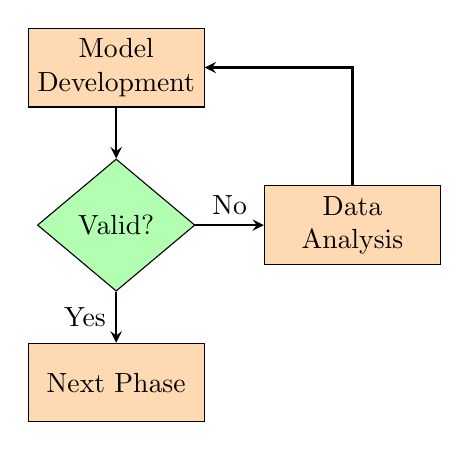
\begin{tikzpicture}[node distance=1.5cm]

                        \node (development) [process] {Model Development};
                        \node (decision) [decision, below of=development, yshift=-0.5cm] {Valid?};

                        \node (analysis) [process, right of=decision, xshift=1.5cm] {Data Analysis};
                        \node (experiments) [process, below of=decision, yshift=-0.5cm] {Next Phase};

                        \draw [arrow] (development) -- (decision);
                        \draw [arrow] (decision) -- node[anchor=east] {Yes} (experiments);
                        \draw [arrow] (decision) -- node[anchor=south] {No} (analysis);
                        \draw [arrow] (analysis) |- (development);

                    \end{tikzpicture}
                }

            \end{figure}

        \end{column}

        \begin{column}{0.5\textwidth}

            Evaluation test cases are dependent on the literature review and the experimental data founds.

            If available, the following metrics will be adopted:

            \begin{itemize}
                \item Droplet size distribution.
                \item Temperature and pressure profiles.
                \item Spray geometry (angle, penetration, and shape).
            \end{itemize}

        \end{column}

    \end{columns}

\end{frame}



\begin{frame}{Phase 2.1 - Experimental Campaign}

    In the optic of gathering as many data as possible, an \textbf{experimental campaign with some preexisting injector in the context of Ammonia combustion in ICE} will be conducted.

    \vspace{9pt}

    \begin{columns}[c, onlytextwidth]

        \begin{column}{0.6\textwidth}

            Main goal: better understand the combustion process of Ammonia in an ICE (\textbf{reactive environment}).

            \vspace{9pt}

            Possible instruments to be used:

            \begin{itemize}
                \item High-speed camera.
                \item Pressure and temperature sensors.
                \item Gas analyzer.
            \end{itemize}

        \end{column}

        \begin{column}{0.4\textwidth}

            \begin{figure}
                \centering
                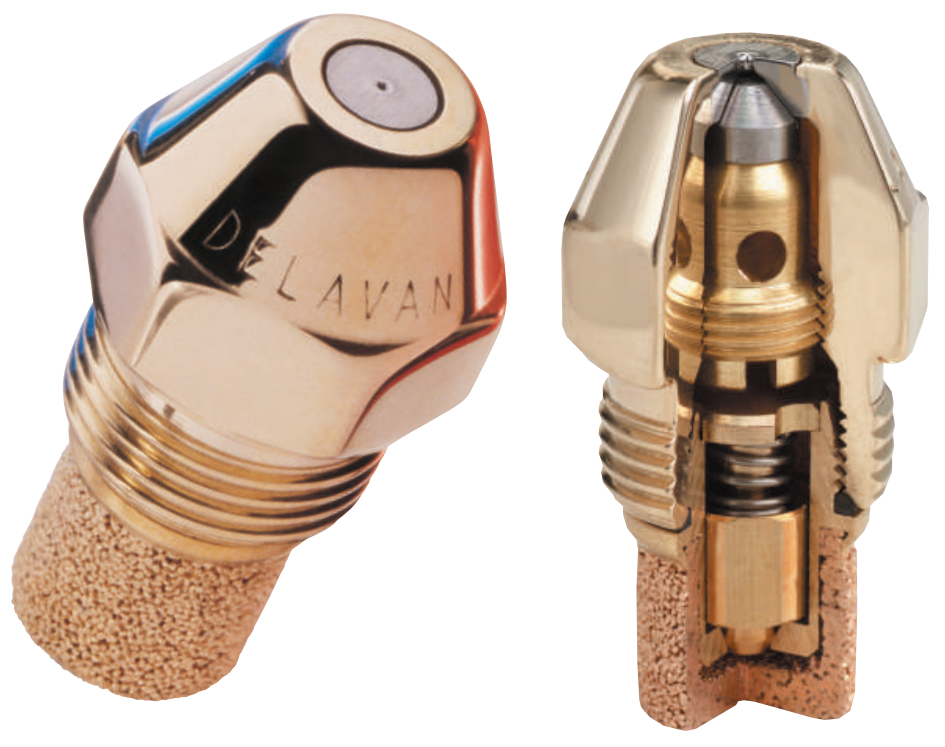
\includegraphics[width=0.9\columnwidth]{img/Delavan-nozzle.png}
                \caption{\texttt{Delavan} hollow cone nozzle that may be adopted.}
            \end{figure}

        \end{column}

    \end{columns}

\end{frame}



\begin{frame}{Phase 2.2 - Data Analysis}

    \begin{columns}[c, onlytextwidth]

        \begin{column}{0.5\textwidth}

            \begin{figure}
                \centering

                \resizebox{0.7\columnwidth}{!}{%
                    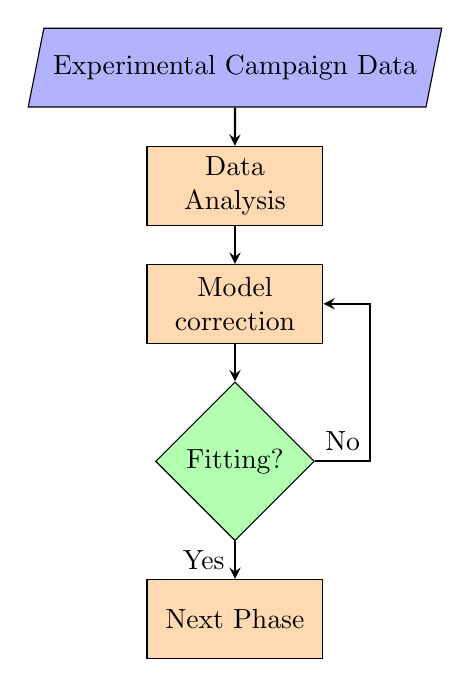
\begin{tikzpicture}[node distance=1.5cm]

                        \node (experiments) [io] {Experimental Campaign Data};
                        \node (analysis) [process, below of=experiments] {Data Analysis};
                        \node (correction) [process, below of=analysis] {Model correction};
                        \node (decision) [decision, below of=correction, yshift=-0.5cm] {Fitting?};
                        \node (design) [process, below of=decision, yshift=-0.5cm] {Next Phase};

                        \draw [arrow] (experiments) -- (analysis);
                        \draw [arrow] (analysis) -- (correction);
                        \draw [arrow] (correction) -- (decision);
                        \draw [arrow] (decision) -- node[anchor=east] {Yes} (design);
                        \draw [arrow] (decision.east) -- node[auto] {No} ++(20pt,0pt) |- (correction.east);

                    \end{tikzpicture}
                }

            \end{figure}

        \end{column}

        \begin{column}{0.5\textwidth}

            For each experimental test, data will be collected and analyzed.

            \vspace{9pt}

            The following analysis methods might be exploited:

            \begin{itemize}
                \item Data visualization.
                \item Machine learning.
                \item Statistical analysis.
            \end{itemize}

        \end{column}

    \end{columns}

\end{frame}



\begin{frame}{Phase 3 - Fuel Injector Design \& Testing}

    After the final model validation, the \textbf{design of the new injector} will follow.

    \vspace{9pt}

    \begin{columns}[c, onlytextwidth]

        \begin{column}{0.5\textwidth}

            As the CAD system, \texttt{CATIA V5} will be used.

            \vspace{9pt}

            The key factors driving our design will be:

            \begin{itemize}
                \item Stable flame inside the combustion chamber
                \item Low-to-zero $\mathrm{NO_x}$ emissions
            \end{itemize}

        \end{column}

        \begin{column}{0.5\textwidth}

            \begin{figure}
                \centering
                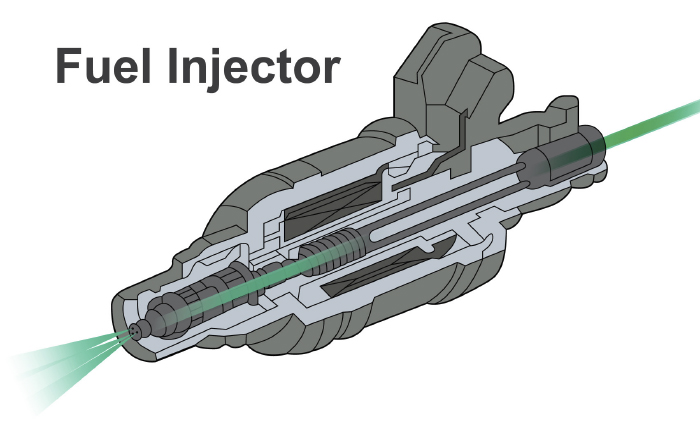
\includegraphics[width=0.9\columnwidth]{img/Fuel-injector.jpg}
            \end{figure}

        \end{column}

    \end{columns}

    \vspace{9pt}

    The new design will be \textbf{tested in a real ICE} and the data collected will be used \textbf{to evaluate its performance}.

\end{frame}
\section{Expected Results}

\begin{frame}{Expected Results}

    To summarize, the expected results of this research are:

    \begin{itemize}
        \item<2-> Phase 1: \textbf<2>{Numerical model of the Ammonia dynamics for non-reactive condition}.
        \item<3-> Phase 2: Set of experimental data and \textbf<3>{numerical model of the Ammonia dynamics for reactive condition}.
        \item<4-> Phase 3: \textbf<4>{Fuel injector design for pure Ammonia combustion}.
    \end{itemize}

    \begin{columns}[t, onlytextwidth]

        \begin{column}{0.28\textwidth}

            \only<2->{
                \begin{figure}
                    \centering
                    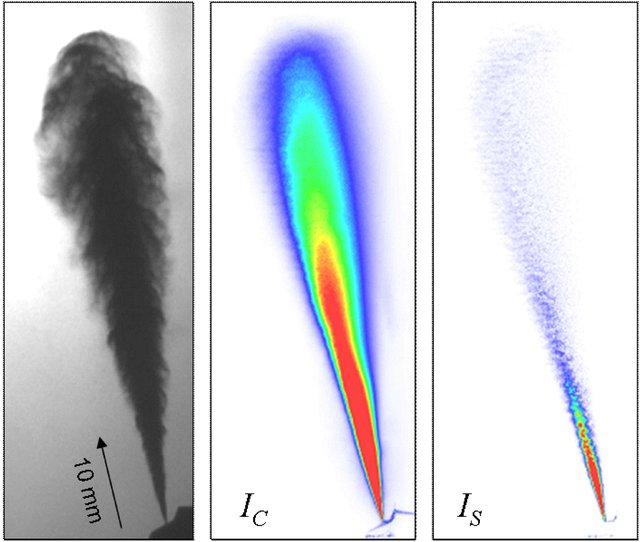
\includegraphics[height=2.6cm]{img/result-phase-1.jpg}
                    \caption{NM\footnotemark[1] (non-reactive condition).}
                \end{figure}
            }

        \end{column}

        \hfill

        \begin{column}{0.28\textwidth}

            \only<3->{
                \begin{figure}
                    \centering
                    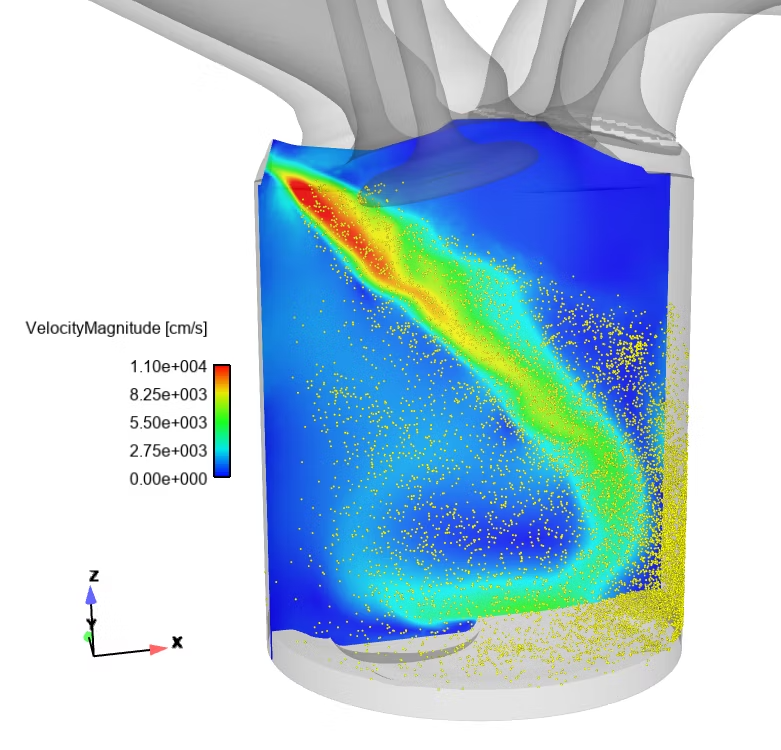
\includegraphics[height=2.6cm]{img/result-phase-2.png}
                    \caption{NM\footnotemark[1] (reactive condition).}
                \end{figure}
            }

        \end{column}

        \hfill

        \begin{column}{0.36\textwidth}

            \only<4->{
                \begin{figure}
                    \centering
                    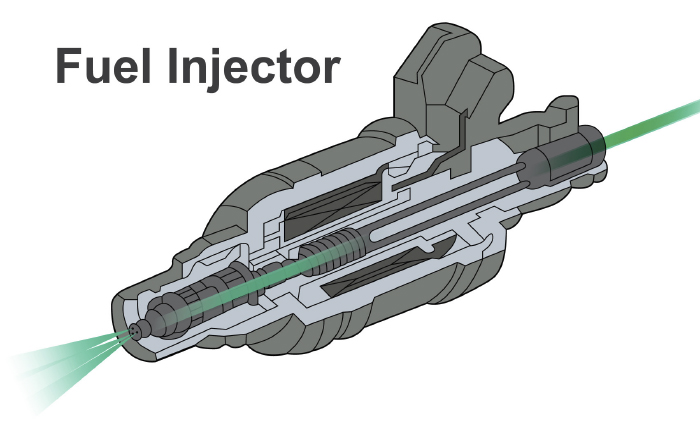
\includegraphics[height=2.6cm]{img/Fuel-injector.jpg}
                    \caption{Fuel injector design.}
                \end{figure}
            }

        \end{column}

    \end{columns}

    \only<2->{\footnotetext[1]{NM: Numerical Model.}}

\end{frame}


\begin{frame}[standout]
    Extra slides
\end{frame}



\begin{frame}{$\mathrm{NO_x}$ Emissions}

    \begin{figure}[H]
        \centering
        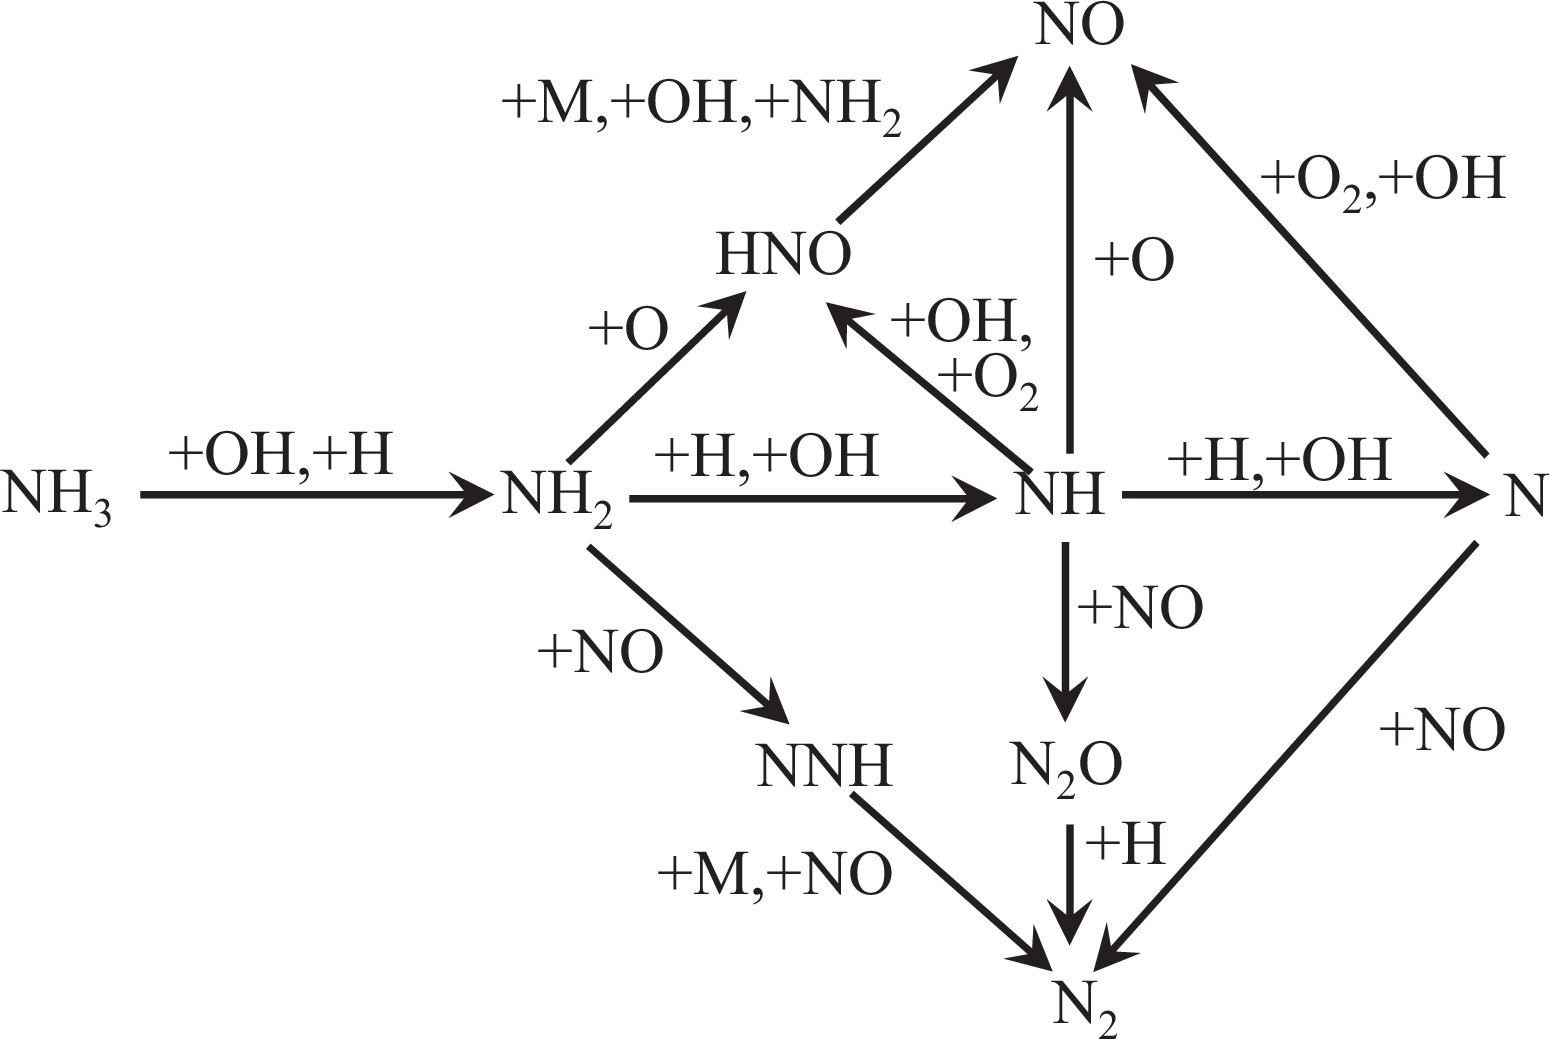
\includegraphics[width=0.6\textwidth]{img/NOx-emission-diagram.jpg}
        \caption{$\mathrm{NH_3}$ oxidation pathway}
    \end{figure}

\end{frame}



\begin{frame}

    More of the different types of NOx emissions

    More of the different types of fuel injectors

    Who uses a suitable replacing combution chamber, what's our target?

\end{frame}

\appendix

\begin{frame}[allowframebreaks]{References}
    \nocite{*}
    \bibliography{references}
\end{frame}

\begin{frame}[standout]
    Questions?
\end{frame}

\begin{frame}[standout]
    Thank you!
\end{frame}

\end{document}